\documentclass{llncs}

\usepackage{color}
\usepackage{colortbl}
\usepackage{epsfig}
\usepackage{listings}
\usepackage{array}
\usepackage{longtable}
\usepackage{hhline}
\usepackage{cite}
\usepackage{boxedminipage}
\usepackage{graphicx}

\newcommand{\notesbox}[1]{
  \noindent\begin{center}\begin{boxedminipage}[h]{0.4\textwidth}{#1}\end{boxedminipage}\end{center}
}

\definecolor{lightgray}{gray}{.95}
\definecolor{darkgray}{gray}{.80}

\lstset{
  lineskip=0.5pt,
  basicstyle=\scriptsize,             % the size of the fonts that are used for the code
  %numbers=left,                      % where to put the line-numbers
  numberstyle=\scriptsize,            % the size of the fonts that are used for the line-numbers
  stepnumber=1,                       % the step between two line-numbers. If it is 1 each line will be numbered
  numbersep=3pt,                      % how far the line-numbers are from the code
  backgroundcolor=\color{lightgray},  % choose the background color. You must add \usepackage{color}
  showspaces=false,                   % show spaces adding particular underscores
  showstringspaces=false,             % underline spaces within strings
  showtabs=false,                     % show tabs within strings adding particular underscores
  frame=none,                         % adds a frame around the code
  tabsize=2,                          % sets default tabsize to 2 spaces
  captionpos=b,                       % sets the caption-position to bottom
  breaklines=true,                    % sets automatic line breaking
  breakatwhitespace=false,            % sets if automatic breaks should only happen at whitespace
  escapeinside={\%}{)}                % if you want to add a comment within your code
}

\hyphenation{op-tical net-works semi-conduc-tor}

\begin{document}

\title{ARC: Automatic Repair of Concurrency Bugs}

\author{Kevin Jalbert, David Kelk, Jeremy S. Bradbury}

\institute{Software Quality Research Group\\
%Faculty of Science (Computer Science)\\
University of Ontario Institute of Technology\\
Oshawa, Ontario, Canada\\
\email{\{kevin.jalbert, david.kelk, jeremy.bradbury\}@uoit.ca}}

\maketitle

\begin{abstract}

Automatic program repair using search-based algorithms has been successfully applied to single-threaded programs. Similar progress has not been made on the automatic repair of concurrent programs. Several challenges exist in concurrent program repair  that are not found in sequential source code: (1) concurrent programs have many possible thread interleavings that make bugs harder to detect and (2) concurrent programs have to contend with complex interaction bugs that not possible in single-threaded source code. In this paper we introduce ARC, a fully automated system for repairing deadlocks and data races in concurrent Java programs. ARC uses a genetic algorithm without crossover to mutate an existing ``buggy'' program searching for a variant of the original program that fixes any deadlocks or data races. 
%The approach works on any Java source code and requires only rudimentary test cases. Annotations, formal specifications or other notations are not required. As only the concurrency mechanisms are targeted the semantic meaning of the program is not changed. As the first phase may introduce unneeded synchronization, a second phase attempts to optimize performance by removing the excess synchronization without sacrificing program correctness. We describe the approach and report on early results.
In addition to introducing ARC, we evaluate it on eight programs from the IBM concurrency benchmark. 


\end{abstract}
\section{Introduction}
\label{sec:introduction}

As computers and mobile devices now ship with more than one processor, programs
must take advantage of multiple processes as we have approached the end of
the\textit{free-lunch}~\cite{SL05}. Parallelism introduces a new class of bugs
and what makes them difficult to find is that they only occur in a small set of
execution interleavings~\cite{MQB07}. Even when a concurrency bug as been
detected, the repair of such a bug may not be apparent to the developer. It is
often the case that there are multiple threads and data accesses occurring at
the same time in different locations within the program.

We propose ARC (\textbf{A}utomatic \textbf{R}epair of \textbf{C}oncurrency
bugs): An automatic technique to repair deadlocks and data races in parallel
Java programs. Formal specifications, annotations and elaborate test suites are
not required. Only the Java source code and test(s) demonstrating the deadlocks
and/or data races are necessary. Evolutionary strategies (ES) are used to
evolve variants of the program until one is found that fixes the bugs in
question.

The use of search-based software engineering (SBSE)~\cite{Har+10} techniques to
automatically repair bugs is not a novel idea~\cite{FNWG09, WNLF09, NWLF09,
WFGN10, GNFW11, LDFW12}. Our proposed approach adapts the original idea of
automatically fixing \textit{sequential} programs to specifically target
\textit{concurrent} programs.

ARC uses ES to iteratively evolve a buggy program into a version that contains
the proper synchronization that resolves the concurrency bug. To evaluate
whether a program is fixed or now ARC takes advantage of the IBM's
ConTest~\cite{EFN+02} tool, which is used to explore different interleavings of
the program under test.

A common criticism in automatic bug repair techniques is large search space,
not to mention that parallelism introduces thread interleavings on top of this.
ARC innately lessens some of these problems due to a few design choices. First,
we limit the algorithm to only fixing deadlocks and data races. Second, ARC
only targets concurrency mechanisms (\texttt{synchronize} statements are added,
removed, and manipulated). Third, we use a specific set of 11 TXL~\cite{CHP91}
operators based on the ConMAn suite~\cite{BCD06} to mutate the concurrent
program.  Finally, ARC only considers shared variables during the mutation
process. By considering these four design choices ARC operates on a limited set
of operators, and possible places where mutation can occur.

We cover background material related to concurrency and evolutionary strategies
in Sect.~\ref{sec:background}. The motivation for ARC along with an example
problem are presented in Sect.~\ref{sec:motivation}. In
Sect.~\ref{sec:approach} we describe the approach ARC uses to evolve a fix for
a concurrency bug using ES. We evaluate the fixing effectiveness of ARC in
Sect.~\ref{sec:experiments} by conducing an experiment using several programs.
Three challenges that ARC faces are identified in Sect.~\ref{sec:challenges}.
Threats to validity are covered in Sect.~\ref{sec:threats}. We describe the
current ongoing research to add a second phase to ARC that attempts to improve
the performance of the found fixes in Sect.~\ref{sec:ongoing}. In
Sect.~\ref{sec:related_works} we mention related works in the field of
automatic bug repair. Finally, future work and conclusions are covered in
Sect.~\ref{sec:future_work} \& Sect.~\ref{sec:conclusion}.

% In ongoing work we are adding a second phase to the system.  It attempts to
% improve performance by shrinking and removing synchronization blocks. As this
% can introduce data races or deadlocks, any mutant decreasing correctness is
% rejected. This second phase is still in development.  In the rest of the paper
% we concentrate on the first phase, bug fixing.

% To the best of our knowledge there has been no previous work using evolutionary
% strategies to fix bugs in concurrent software. There has been work involving
% the correction of concurrency bugs using self-healing~\cite{LVK08}. From the
% paper, \textit{The healing techniques based on influencing the scheduling do
% not guarantee that a detected problem will really be completely removed, but
% they can decrease the probability of its manifestation.} In contrast ARC is an
% off-line technique that fixes bugs by modifying the source code.

% The main contributions of this paper are:

% \begin{itemize}

% \item An algorithm to create fixes for deadlocks and data races in concurrent Java
% programs. Only the source code and tests demonstrating the bugs are necessary.
% To the best of our knowledge this is the first approach to fix both kinds of
% bugs in Java programs.

% \item Methods to constrain the search space: First, by specifically targeting
% synchronization mechanisms. Second, by using a limited number of TXL operators
% to transform the Java source.  Third, by targeting the variables used by multiple
% threads and ignoring the rest.

% \end{itemize}

\section{Background}
\label{sec:background}

\subsection{Concurrency Bugs}
\label{sec:concurrency}

% Concurrency is the act of having multiple threads executing in parallel.
% Concurrent programs are able to exploit multi-core systems where threads are
% distributed across each of the CPUs to increase performance.

%Concurrency introduces a new class of bugs, the \textit{heisenbugs}. Due to concurrent access to shared memory, threads are able to cause \textit{data
%races} and \textit{deadlocks}.

Data races and deadlocks are two of the most common concurrency bugs. A \textbf{data race} can be defined as: \textit{``\ldots two or more concurrent threads access a shared variable and when at least one access is a write, and the threads use no explicit mechanism to prevent the access from being simultaneous.''}~\cite{LSW07}. A \textbf{deadlock} can be defined as: \textit{``\ldots a situation where two or more processes are unable to proceed because each is waiting for one of the others to do something in a deadlock cycle \ldots} For example, a deadlock can occur when one thread in a program holds a lock that another thread desires and vice-versa''~\cite{LSW07}.

Improper synchronization in concurrent Java programs allows data races and deadlocks to occur. 
%ARC attempts to fix these bugs by evolving a program that contains proper synchronization.
These bugs are extremely difficult to detect due to the non-deterministic nature of how threads are interleaved (i.e., the way the system schedules threads). Various techniques are available to detect concurrency bugs such as static analysis~\cite{NA07,NPSG09,HP04}, stress testing~\cite{HSU03}, dynamic analysis~\cite{JNPS09,EFN+02}, and model checking~\cite{BHPV00,RDH03,OM03,MQB07,Holz97,JM04,HP00}.
% TODO Possibly trim out some of the techniques for bug detection?

\subsection{Evolutionary Strategies}
\label{sec:evolutionary_strategies}

ES is an example of a heuristic search algorithm and shares some similarities  with the most commonly referenced heuristic search technique, the genetic algorithm (GA)~\cite{GA92}. Due to space limitations, we will now provide only a brief outline of ES.

A standard GA is population based, uses mutation, crossover and a fitness function to evolve solutions to problems. A proposed solution to the problem is encoded as an individual of the population. Each individual is evaluated by a fitness function, which is an equation that determines how close the individual is to the solution. The more fit a individual's solution is, the greater the chance it will pass it's genetic material (i.e., part of the solution) on to the next generation.
%\textit{Selection pressure preferentially selects better solutions.}
Crossover mixes the individuals to produce new ones while mutation injects fresh information in to the population so it does not become stagnant.

ES is a simpler form of search than a genetic algorithm. A population of proposed solutions is generated and mutated each generation. Crossover and selection aren't used. Every individual's fitness is evaluated every generation. ES end when a predetermined fitness is reached, after a set number of generations have passed or after a search budget is exhausted.

ARC uses an ES instead of a GA because intuitively, crossover does not seem to fit well with the problem. In particular, using crossover to mix two states of a program in relation to repairing concurrency could lead to more troubles in regards to merging the two code bases. Our rational is to use ES and leave crossover/selection as possible future work.

\section{Motivation}
\label{sec:motivation}

Recall that concurrency bugs often are the result of multiple code fragments in different threads interacting in an undesirable way. The multiple code fragments involved in a concurrency bug can be in different units of code and can therefore be difficult to locate, making the appropriate fix not always clear. Once solution to this problem is to use concurrency anti-patterns that provide a definition, problem, context and solution for concurrency bugs~\cite{BJ09,FKLV12}. Unfortunately, the use of anti-patterns still requires the programmer to have identified the concurrency bug before assisting with repairing the bug.

\begin{figure}[t!]
\begin{minipage}{5cm}
\footnotesize{\textbf{Buggy Program:}}
\begin{lstlisting}[language=Java, morekeywords={synchronize}]
write(int var1){
  ... // Expensive loop
  data = var1;
  ... // Database query
}

int public read(){
  return data;
}
\end{lstlisting}
\end{minipage}\hfill
\begin{minipage}{5cm}
\footnotesize{\textbf{Fixed Program:}}
\begin{lstlisting}[language=Java, morekeywords={synchronize}]
synchronize write(int var1){
  ... // Expensive loop
  data = var1;
  ... // Database query
}

int synchronize read(){
  return data;
}
\end{lstlisting}
\end{minipage}
\caption{A developer first synchronizes the \texttt{read} function, yet the bug
still exists. Synchronizing the \texttt{write} method as well fixes the bug.}
\label{fig:fixed_sample_datarace}
\end{figure}

\begin{figure}[t!]
\begin{minipage}{5cm}
\footnotesize{\textbf{$1^{st}$ Optimization on Fix:}}
\begin{lstlisting}[language=Java, morekeywords={synchronize}]
public write(int var1){
 ... // Expensive loop
 synchronized(this){
   data = var1;
   ... // Database query
 }
}

int synchronize read(){
 return data;
}
\end{lstlisting}
\end{minipage}\hfill
\begin{minipage}{5cm}
\footnotesize{\textbf{$2^{nd}$ Optimization on Fix:}}
\begin{lstlisting}[language=Java, morekeywords={synchronize}]
public write(int var1){
 ... // Expensive loop
 synchronized(this){
   data = var1;
 }
 ... // Database query
}

int synchronize read(){
 return data;
}
\end{lstlisting}
\end{minipage}
\caption{A developer shrinks the critical region to exclude the expensive loop (Optimization 1). Next, a developer shrink the critical region again to exclude the database query (Optimization 2).}
\label{fig:optimized_sample_datarace}
\end{figure}


To illustrate the challenges of concurrency bug repair we now consider an example of a data race bug and how a developer might fix it. In the left part of Fig.~\ref{fig:fixed_sample_datarace} the \texttt{read} and \texttt{write} method access a shared variable. A very simple data race exists because there is no atomic access to the \texttt{data} variable during the concurrent reading or writing.
%Both methods are involved in the data race, and it is because of the interactions between these methods the data race is possible.
A possible repair involves synchronizing both accesses as shown in the right part of Fig.~\ref{fig:fixed_sample_datarace}. Note that synchronizing one method alone does not completely fix the bug in this case.

% Phase 2 - the optimization phase in development - addresses the issue of unnecessarily synchronizing the ``expensive loop'' and ``database query''.

The solution in the right part of Fig.~\ref{fig:fixed_sample_datarace} is far from ideal. It forces other threads to wait unnecessarily while the write method works in the loop and database sections. An optimization is to shrink the critical region (the synchronized statements) to only guard access to the shared variable as shown in Fig.~\ref{fig:optimized_sample_datarace}.
%From a developer's standpoint there is a lot of work involved in creating a fix for parallel bugs as multiple, unrelated changes are not uncommon. 
In total two changes are required to functionally fix the example program, and two additional changes are required to improve the non-functional performance. % An ideal fix only requires two changes which minimizes the time spent in the critical region. 
Currently, ARC is capable of finding a fix for a concurrency bug, it does not make an attempt at ensuring the fix is close to optimal (finding the best fix from a performance standpoint is ongoing research and is explained in Sect.~\ref{sec:ongoing}).

%Automated tools in software testing and debugging are needed as they have the potential to reduce the vast amount of resources spent on software testing (upwards to \$59.5 billion)~\cite{RTI02}. ARC provides an automated approach to fixing the \textit{functionality}, and then optimizing the \textit{non-functional} performance of programs with deadlocks and data races.

\section{ARC's Approach}
\label{sec:approach}

%ARC aims to automatically repair concurrency bugs like the one presented in
%Sect.~\ref{sec:motivation}.

% A high-level overview of ARC's approach is presented in Fig.~\ref{fig:process}.

There are two inputs to ARC: A ``buggy'' concurrent Java program and a JUnit test
suite. The test suite is necessary as it acts as an oracle to determine if bugs still exists in the program. One limitation of ARC (and of other
related automatic bug fixing techniques mentioned in
Sect.~\ref{sec:related_works}) is that it can only fix bugs detectable by the
test suite.

% \begin{figure}[h]
%   \centering
%   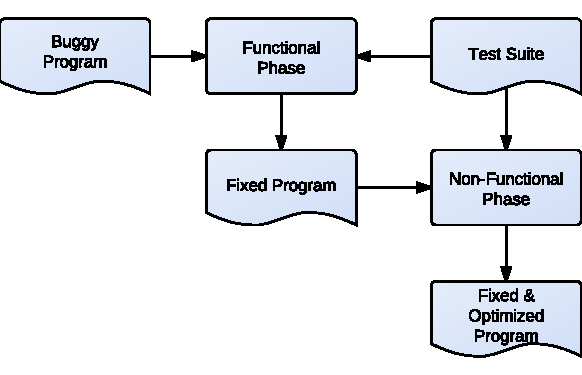
\includegraphics[width=7.0cm]{figures/process.pdf}
%   \caption{High Level Overview of ARC's Repair and Optimization Process}
%   \label{fig:process}
% \end{figure}

%ARC's complete approach is accomplished in two phases, the \textit{Functional
%Phase} and the \textit{Non-Functional Phase}. Both are similar in terms of the
%steps they follow, with slight variations to accomplish different goals. The
%first phase attempts to fix the buggy program while the second attempts to
%optimize its performance.

The following sections detail the fixing process as shown in
Fig.~\ref{fig:phases_internals}. We describe each step in the process in the order they occur. The key aspect of ARC's approach occur in the mutation and evaluation steps.

\begin{figure}[t!]
  \centering
  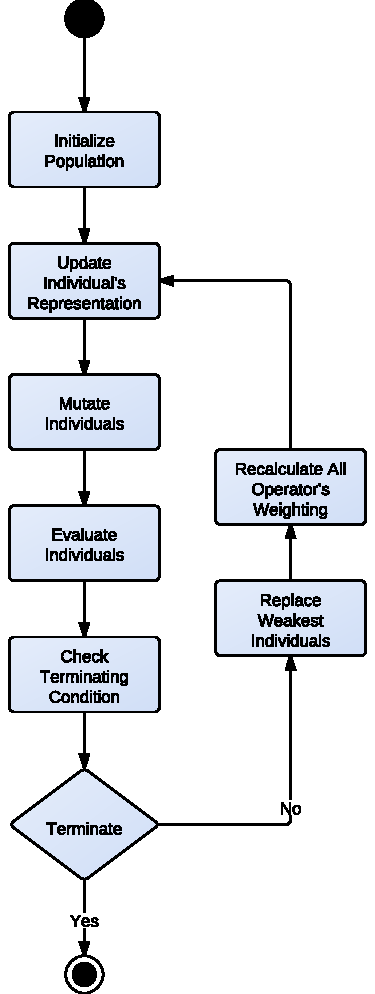
\includegraphics[width=7cm]{figures/phases.pdf}
  \caption{Detailed view of ARC's approach to concurrency bug repair}
  \label{fig:phases_internals}
\end{figure}

\subsection{Update Population}
\label{sec:update_population}

In the first step in the ARC approach the population of individuals is updated. For each
individual the previous generation (or the original program if ARC is just
starting) is copied to the current generation. Each individual contains their
own version of the program and the different versions evolve independently of each other.

% For the non-functional phase ARC has already produced the fixed
% program so each individual receives a copy of the fixed program to optimize.

\subsection{Update Individual's Representation}
\label{sec:update_individual_representation}

At this step ARC updates the individual's representation, which is accomplished
by generating the possible mutations from the current generation's program (which
is copied from the previous generation).

%Internally ARC keeps track of the mutants using a
%representational form as shown in Table~\ref{tbl:individual_representation}. As
%there exists multiple types of mutations, individuals are represented using a
%2-dimensional array of the mutation operators and the number of mutation
%instances generated.

%\begin{table}[h]
%\begin{center}
%\caption{An example representation of an individual, each 0 represents an
%instance of that mutation type that has been generated. It is possible for up
%to $n$ mutation operators with no-limit to the number of instances per
%operator.}
%\begin{tabular}{|l|l|}
%\hline
%\textbf{Operator} & \textbf{Instances}\\
%\hline
%Mutation 1 & 0\\
%\hline
%Mutation 2 & 0 0 0\\
%\hline
%Mutation 3 & --\\
%\hline
%\ldots & \ldots\\
%\hline
%Mutation $n$ & 0 0\\
%\hline
%\end{tabular}
%\label{tbl:individual_representation}
%\end{center}
%\end{table}

\begin{table}[t!]
\caption{Set of mutation operators used by ARC.}
\begin{center}
\begin{tabular}{|l|l|c|c|}
\hline
\textbf{Operator Description} & \textbf{Acronym} \\
\hline
Add synchronized around synchronized & ASAS \\
\hline
Add synchronized around variable & ASAV \\
\hline
Add synchronized in method header & ASIM \\
\hline
Add synchronized around method & ASM  \\
\hline
Change synchronized order & CSO  \\
\hline
Expand synchronized before & EXSB  \\
\hline
Expand synchronized after & EXSA  \\
\hline
Remove synchronized around synchronized & RSAS  \\
\hline
Remove synchronized around variable & RSAV  \\
\hline
Remove synchronized in method header & RSIM  \\
\hline
Remove synchronized around method & RSM  \\
\hline
\end{tabular}
\label{tbl:operators}
\end{center}
\end{table}

\begin{figure}[t!]
\vspace{2mm}
\begin{minipage}{5cm}

\footnotesize{\textbf{ Program $P$:}}
\begin{lstlisting}[language=Java, morekeywords={synchronize}]
obj.write(var1);
synchronized(lock){
  myHash.remove(var1);
}
\end{lstlisting}
\end{minipage}\hfill
\begin{minipage}{5cm}
\footnotesize{\textbf{ Program $P'$:}}
\begin{lstlisting}[language=Java, morekeywords={synchronize}]
synchronized(lock){
  obj.write(var1);
  myHash.remove(var1);
}
\end{lstlisting}
\end{minipage}

\caption{An example of the EXSB (expand synchronization before) mutation
operator.}
\label{fig:EXSB_example}
\end{figure}

The set of mutation operators ARC uses are listed in Table~\ref{tbl:operators},
and have mostly been derived by reversing the ConMAn operators~\cite{BCD06}. The ConMAn operators are used in mutation testing to create bugs while the ARC operators are used to fix bugs. The ARC operators are implemented in 
TXL~\cite{CHP91} using pattern matching and replacement rules. An example of one of the ARC operators, 
EXSB, is shown in Fig.~\ref{fig:EXSB_example}. Each mutant
that is generated from the program creates a new mutant instance for that
individual of the mutation type.

% Original table with functional and non-functional
%\begin{table}[h]
%\caption{Set of mutation operators used by ARC. Each mutation operator is
%active during the indicated phases.}
%\begin{center}
%\begin{tabular}{|l|l|c|c|}
%\hline
%\textbf{Operator} & \textbf{Acronym} & \textbf{Functional} & \textbf{Non-Functional}\\
%\hline
%Add synch. around synch. & ASAS & $\surd$ &\\
%\hline
%Add synch. around variable & ASAV & $\surd$ &\\
%\hline
%Add synch. in method header & ASIM & $\surd$ &\\
%\hline
%Add synch. around method & ASM & $\surd$ &\\
%\hline
%Change synch. order & CSO & $\surd$ &\\
%\hline
%Expand synch. before & EXSB & $\surd$ &\\
%\hline
%Expand synch. after & EXSA & $\surd$ &\\
%\hline
%Remove synch. around synch. & RSAS & $\surd$ & $\surd$\\
%\hline
%Remove synch. around variable & RSAV & $\surd$ & $\surd$\\
%\hline
%Remove synch. in method header & RSIM & $\surd$ & $\surd$\\
%\hline
%Remove synch. around method & RSM & $\surd$ & $\surd$\\
%\hline
%Shrink synch. before & SHSB & & $\surd$\\
%\hline
%Shrink synch. after & SHSA & & $\surd$\\
%\hline
%\end{tabular}
%\label{tbl:operators}
%\end{center}
%\end{table}

% Modified table of functional only operators


As ARC mutates synchronization aspects of programs, the mutations themselves
can alter the occurrence of future mutations. This causing the search space of
possible mutations to potentially changes in every generation.

% Thus ARC must update the representation according to the latest state of the
% program's source code each generation.

\subsection{Apply a Mutation to an Individual}
\label{sec:mutate_individuals}

Once all mutants are generated for each individual, ARC selects a type of
mutation (e.g. EXSB) and then an instance of it (e.g. 4$^{th}$ mutant
generated) from those available. The selected mutation is applied and becomes
the current generation's code. ARC at this point will re-compile the project to
ensure that the mutation consists of valid syntax. In the situation that the
compilation fails another mutation type and instance is selected until a valid
combination is found.

ARC can leverage historical information about previous evaluations of the
mutation operators along with information about the current dominating bug type
found during testing. We use a weighted heuristic to select the mutation operator. Specifically, previous mutation operator evaluations and dominating bug types add weight to operators that
have been successful in the past, as well as to select operators that appear to
reduce the occurrences of either deadlocks or data races more often. This
heuristic is further detailed in
Sect.~\ref{sec:recalculate_operator_weighting}. Currently, mutation operator selection
is weighted but the mutant instances are selected randomly with equal
probability.

\subsection{Evaluate Individuals}
\label{sec:evalute_individuals}

A mutation may be beneficial, destructive or benign. We must evaluate it to
determine it's effect on the program. A key problem in evaluating mutants is the unpredictability of
thread interleavings. If a concurrency bug appears in only a few possible interleavings, how can we gain
confidence that a proposed fix actually works? 

ARC uses IBM's ConTest tool~\cite{EFN+02} to instrument the software under repair by injecting noise into the
program. The injected noise causes threads to randomly delay at different times during execution,
effectively causing each execution of the program to explore a different interleaving. By running the instrumented version of the program multiple times we gain more confidence that a larger set of the interleavings
are explored. Running the instrumented program multiple times is the most time
consuming aspect of ARC.

The number of successful ConTest executions are used to determine fitness:

\begin{footnotesize}
\begin{center}
$functional\ fitness(P) = (s \times sw) + (t \times tw)$
\end{center}
\end{footnotesize}
\begin{scriptsize}
\begin{center}
$s = \#\ of\ successful\ executions$ \\
$sw = success\ weighting$ \\
$t = \#\ of\ timeout\ executions$ \\
$tw = timeout\ weighting$
\end{center}
\end{scriptsize}

\noindent In determining fitness we consider both a successful execution and a timeout as positive factors. Timeouts are considered positive because given more time an execution that times out may result in a successful execution. We weight timeouts less than a successful execution as it could still result in a bug.

If ARC finds an individual that achieves 100\% successful executions, we need
to ensure it is truly a fix. It is possible that a proposed solution could
still contain a concurrency bug that escaped detection because the interleaving that exhibits the bug was not encountered by ConTest. To increase our confidence that a fix is correct we run ConTest
an additional number of times if all of the tests passed for the previous executions. The number of additional ConTest executions is usually some multiple of the previous number of runs. If the fix still holds even after this additional testing we feel confident the solution is indeed a true solution. If any of the additional executions fail,
the proposed fix is rejected and the evolutionary process continues.

\subsection{Check Terminating Condition}
\label{sec:check_terminating_condition}

ARC continues to evolve and evaluate individuals until
%some terminating condition is met. The following conditions are for the functional phase:
a solution is found or the
generational limit is reached. If a solution is found ARC outputs the modified program for the user to examine.
%The following conditions are for the non-
%functional phase: The population has converged (no improvement has been seen in
%$x$ generations), no more mutations are generated, or the generational limit is
%hit.

\subsection{Replace Weakest Individuals}
\label{sec:replace_weakest_individuals}

With any evolutionary algorithm it is entirely possible for an individual to
stray down a path leading to little or no improvement. To encourage individuals
to explore more fruitful areas of the state space we employ a replacement
strategy that replaces the lower $w$ percentage of individuals with a random
individual from the upper $x$ percent or the original buggy program with $y$
percent chance. These replacements only occur after an individual has
underperformed for $z$ generations. We believe the \textit{competent programmer
hypothesis}~\cite{ABD+79} applies so the corrected program isn't very far away
in the search space from the original buggy program.
%Therefore we provide a chance for an under-performing individual to reset
%back the initial state to allow the individual to explore from the starting
%point again.

\subsection{Recalculate All Operator's Weighting}
\label{sec:recalculate_operator_weighting}

As mentioned in Sect.~\ref{sec:mutate_individuals} ARC utilizes a heuristic
approach in selecting the mutation operator. A sliding window of $n$
generations is used to determine the success of previously applied mutation
operators. Operators that improve fitness are weighted more heavily and are
more likely to be selected. A sliding window is used to prevent dominance of
operators and to allow for flexibility in changing the weightings based on
recent history. The weighting is designed to ensure the chance of selecting an
operator is always greater than zero regardless of their performance.
%To ensure this approach is up to date the current weighting for
%each operator is recalculated based on the new feedback received from the
%population.
We consider a separate weighting for data races and deadlocks to remain
accurate in the use of this heuristic based on the current bug ARC is trying to
fix.

\section{Experiments}
\label{sec:experiments}

% Due to the ARCs heuristic nature it is entirely possible for a program to
% perform better or worse then it did originally. We are interested in both ARCs
% ability to find fixes and ARCs effect on performance of solutions found.

\subsection{Experimental Setup}
\label{sec:experimental_setup}

We evaluate ARC's ability to repair concurrency bugs by conducing an experiment
to gather preliminary results. The 8 buggy programs we chose come from a
subset of the IBM Concurrency Benchmark~\cite{EHSU06}. Our selection criteria
was to pick a subset of programs containing bugs that ARC has the
capability of fixing based on the set of mutation operators. For example, we
ignored programs that used some of the newer concurrency structures from Java 5. We
also included some programs that we identified that ARC could not fix as a
sanity check.

Unfortunately, none of the programs contained the JUnit test suite that ARC requires.
We manually created JUnit test suites without altering the programs and their
bugs's behaviour\footnote{One incorrect program was fixed so that it properly
exhibited its concurrency bug.}. Each test suite consists of three unit tests
each with a different \textit{level} of concurrency\footnote{IBM Concurrency Benchmark
programs have an argument that controls the number of threads that are used in
execution.}. Source code details on the programs are presented in
Table~\ref{tbl:used_programs}

% TODO Maybe just remove the Bug Pattern (as it would need more explanation)
\begin{table}[h]
\caption{The set of programs used to evaluate ARC. The test suite for each
program is excluded from these values.}
\begin{center}
\begin{tabular}{|l|r|r|l|l|l|}
\hline
\textbf{Program} & \textbf{SLOC} & \textbf{Classes} & \textbf{Bug Type} & \textbf{Can Fix?} & \textbf{Bug Pattern}\\
\hline
account & 165 & 3 & Data Race & Yes & NoLock\\
\hline
accounts & 75 & 2 & Data Race & Yes & NonAtomicAssumedAtomic\\
\hline
airline & 93 & 1 & Data Race & No & Interference\\
\hline
%allocation & 165 & 3 & Data Race & Yes & TwoStageAccess\\
%\hline
%bubble & 246 & 4 & Data Race & No & NonAtomicAssumedAtomic,\newline OrphanedThread\\
%\hline
bubblesort2 & 104 & 2 & Data Race & No & Initialization-Sleep\\
\hline
buffer & 319 & 5 & Data Race & No & NotifiyInsteadOfNotifyAll\\
\hline
%bufwriter & 170 & 5 & Deadlock & Yes & NoLock\\
%\hline
deadlock & 109 & 2 & Deadlock & Yes & Deadlock\\
\hline
lottery & 157 & 2 & Data Race & No & NonAtomicAssumedAtomic,\newline NoLock, BlockingCriticalSection\\
\hline
%mergesort & 281 & 2 & Data Race & No & NonAtomicAssumedAtomic\\
%\hline
pingpong & 143 & 4 & Data Race & Yes & NonAtomicAssumedAtomic\\
\hline
\end{tabular}
\label{tbl:used_programs}
\end{center}
\end{table}

ARC was designed to be flexible in terms of the parameters that can be
configured. Table~\ref{tbl:used_parameters} lists and describes each parameter,
including the values selected for evaluation. Values were selected based on our
experience with ARC. The selected parameters allowed for 10 ConTest executions
to occur to evaluate each individual at each generation. If a potential
solution is found, the validation of that potential solution will execute an
addition 150 ConTest executions (10 ConTest Runs $\times$ Validation Mult. of
15).

% TODO Maybe reduce this to the common ES parameters?
\begin{table}%[h]
\caption{The set of parameters that ARC uses along with their descriptions and
used values for the experimentations.}
\begin{center}
\lstset{basicstyle=\scriptsize}
\begin{tabular}{|l|l|r|}
\hline
\textbf{Parameter} & \textbf{Description} & \textbf{Value}\\
\hline
Project Test MB & The amount of memory allocated for the testing & 2000\\
\hline
ConTest Runs & Test suite executions per gen. per member & 10\\
\hline
Validation Mult. & Multiplier on ConTest runs when validating the functionality & 15\\
\hline
Timeout Mult. & Time multiplier for ConTest before timeout & 20\\
\hline
Evolution Gen & Maximum number of generations in fixing phase & 30\\
\hline
Evolution Population & Population size for the evolutionary strategy & 30\\
\hline
Replace Lowest \% & Lowest $n$\% of population replaced & 10\\
\hline
Replace With Best \% & Replace underperfomer with best individual $n$\% of the time & 75\\
\hline
Replace min turns & Minimum time underperforming & 3\\
\hline
Replace Interval & Every $n$ generations, underperformers are replaced & 5\\
\hline
Ranking Window & Size of sliding window for operator weighting & 5\\
\hline
Success Weight & The weighting applied for successful executions & 100\\
\hline
Timeout Weight & The weighting applied for timeout executions & 50\\
\hline
Improv. Window & Size of window for convergence check & 10\\
\hline
Avg. Fit. Delta & Minimum average fitness improvement required & 0.01\\
\hline
Best Fit. Delta & Minimum best fitness improvement required & 1\\
\hline
\end{tabular}
\label{tbl:used_parameters}
\end{center}
\end{table}

\subsection{Experimental Results}
\label{sec:experimental_results}

Each program was run through ARC a total of 5 times using the parameters
described in Table~\ref{tbl:used_parameters} and Programs in
Table~\ref{tbl:used_programs}. Results for each program is summarized in
Table~\ref{tbl:summary_results}.

\begin{table}%[h]
\caption{Summary of the results of running the programs
(from Table~\ref{tbl:used_programs}) through ARC 5 times.}
\begin{center}
\lstset{basicstyle=\scriptsize}
\begin{tabular}{|l|l|l|}
\hline
\textbf{Program} & \textbf{Gen. Fix Found} & \textbf{Time Taken (h:m:s)}\\
\hline
account & 4, 15, 4, 1, 1 & 0:19:53, 1:08:30, 0:19:54, 0:06:39, 0:06:29\\
\hline
accounts & 1, 1, 1, 1, 1 & 2:02:57, 2:08:11, 2:05:31, 2:10:18, 2:36:24\\
\hline
airline & --, --, --, --, -- & 3:58:07, 3:56:19, 3:49:34, 3:53:14, 3:57:51\\
\hline
%allocation & TO, TO, TO, 3, TO & --, --, --, 22:39:6, --  \\
%\hline
%bubble & 28, & 5:20:33, \\
%\hline
bubblesort2 & 2, 2, 3, 2, 2 & 3:15:06, 5:11:04, 5:53:14, 6:13:16, 7:05:32 \\
\hline
buffer & --, --, --, --, -- & 4:43:50, 4:45:12, 5:07:03, 4:58:27, 5:02:30\\
\hline
%bufwriter & TO, TO, TO, TO, TO & --, --, --, --, --\\
%\hline
deadlock & 1, 1, 1, 1, 1 & 0:06:45, 0:05:43, 0:06:45, 0:05:40, 0:07:51\\
\hline
lottery & 3, 4, 2, 1, 2 & 2:19:18, 2:43:18, 1:54:00, 1:05:27, 1:28:39\\
\hline
%mergesort & & \\
%\hline
pingpong & 1, 1, 1, 1, 1 & 0:39:57, 0:12:47, 0:46:21, 0:46:16, 0:42:02\\
\hline
\end{tabular}
\label{tbl:summary_results}
\end{center}
\end{table}

As we can see from the results, the time taken to find a fix range from
about 6 minutes to almost a whole day. ARC is currently not an efficient process
as it is under-optimized in many aspects. The main bottle-neck in terms of time
and resources within ARC is the repeated number of ConTest executions. ConTest
instrumented a program with random noise that negatively effects the performance 
of the execution.  The \textit{Timeout Multiplier} in Table~\ref{tbl:used_parameters} allows ARC to wait up to 20 times the normal execution time for the program under test to complete due to the noise. 

% TODO Add discussion of ARCs fix finding capabilities. Does it find fixes for
% the programs we figured ARC should be able too, did it find fixes for those
% we didn't thing it could (how?). Any comment on the generation fixes were
% found on?

% The state spaces of the found fixes, we would expect the larger state space
% programs to have their fixes found later. This does not seem to be the case.
% allocation 76
% deadlock - 89
% accounts - 102
% bubblesort2 - 103
% pingpong - 123
% account - 163
% bubble - 178
% lottery - 188

\section{Threats to Validity}
\label{sec:threats}

The main threat to validity with respect to our experimental evaluation of ARC is related to external validity -- our ability to generalize our results. Although we have used third-party programs in our experiment, all of the programs are relatively small in size and are not representative of large-scale concurrent software. Furthermore, the test sets for this programs were created by us and are not as comprehensive as those maintained with mature software systems. In the future, we plan to address this threat by conducting further experiments with larger open source concurrent software systems.
\section{Next Steps in ARC Approach}
\label{sec:ongoing}

ARC may introduce unnecessary concurrency during the fixing process. We are
experimenting with and implementing a second phase (non-functional phase) where
the same kind of evolutionary strategy attempts to optimize the program by
shrinking and removing concurrency blocks (solves issues as illustrated in
Fig.~\ref{fig:optimized_sample_datarace} back in Sect.~\ref{sec:motivation}). A
new fitness function would be required for this non-functional phase:

\begin{footnotesize}
\begin{center}
$non-functional\ fitness(P) = \frac{worst\ score}{[sig_t \times unc(t)] + [sig_c \times unc(c)]}$
\end{center}
\vspace{0.1cm} \textit{Where:} \vspace{0.1cm}
\end{footnotesize}
\begin{scriptsize}
\begin{center}
$unc(x) = \frac{(x_{max} - x_{min})}{x_{avg}}$ \\ \vspace{0.2cm}
$
 sig_t = \left\{
 \begin{array}{l l}
   t/c & \quad if\ t\ > c \\
   c/t & \quad if\ c\ > t \\
 \end{array} \right.
$ \\ \vspace{0.2cm}
$
 sig_s = \left\{
 \begin{array}{l l}
   c/t & \quad if\ t\ > c \\
   t/c & \quad if\ c\ > t \\
 \end{array} \right.
$ \\
\end{center}
\end{scriptsize}


\noindent The proposed fitness function combines the real time ($t$ in fitness function) required for an execution and the number of
voluntary context switches ($c$ in fitness function) made.  Voluntary context switches is the number of times a thread voluntarily gives up control of the CPU. By minimizing unnecessary synchronization the number of context switches should
decrease along with the real time taken. We plan to acquire a baseline of the
time and context switches from the newly fixed program by running it a large
number of times and averaging the values acquired. This baseline is then used in
the fitness function to evaluate relative improvements from the fixed
unoptimized program. Note that the fitness function would adjust based on the
significance and uncertainty of both variables (to be fair in situations where
either variable is under-represented).

Removing and reducing synchronization runs the risk of introducing new bugs
into the program. Before every non-functional phase's evaluation we need to
ensure that no bugs are present, thus we re-run the first phase's evaluation
with the multiplier on the number of runs. If any deadlocks or data races are
encountered the proposed optimization is rejected and this individual is reset
to the previous generation. After ARC validates the proposed optimization
additional runs are conducted without using ConTest (avoiding the inclusion of
random noise) to obtain the values required for the non-functional fitness
function. Currently, we have implemented most of this proposed extension but have not conducted any empirical evaluation.

\section{Related Works}
\label{sec:related_works}

%There are a number of approaches to automatically hide or fix bugs in programs.

With respect to sequential programs, several approaches to program repair have been proposed in the literature. For example, co-evolutionary competition between programs with bugs and between test cases is used
in~\cite{AY08, Arc08, WT10}. Both approaches require formal specifications and
both use genetic programming to evolve fixes. Alternatively the work in~\cite{FNWG09, WNLF09, NWLF09, WFGN10, GNFW11,
LDFW12} requires no formal specifications. Instead, test cases are used
to demonstrate the bug and describe the desired functionality that must be
preserved. To address the limitations of the previous approach they introduce
two innovations: First, they assume the bug is written correctly in another
part of the program. Second, they determine the error path on which the bug
occurs and target those statements specifically for repair. Together these
additions constrain the state space enough that the framework can fix real bugs
in real programs.

With respect to concurrent programs there are several examples of related work. Similar to the work done here,~\cite{KLT+07, LVK08} uses ConTest to heal data
races. Healing a program is not the same as repairing a program -- \textit{``The healing techniques based on influencing the scheduling do not guarantee that a detected problem will really be completely removed, but they can decrease the probability of its manifestation.''}~\cite{LVK08}. SAT solving is used in~\cite{AY07}  to repair shared memory concurrent programs
``w.r.t. CTL specifications'' where processes atomically read, write one shared
variable at a time. This work requires the concurrent program and a formal temporal logic
specification. Single variable atomicity violations are repaired in~\cite{JSZL+11}. This approach combines dynamic bug analysis, patch creation and merging and dynamic testing but is more limited than our approach with respect to the kinds of bugs that can be repaired.
\section{Conclusions and Future Work}
\label{sec:conclusion}


We have successfully demonstrated using an evolutionary strategy to automatically repair concurrent Java programs. Our approach overcomes several of the existing challenges of program repair including: (1) concurrent programs can have many possible thread interleavings which can make bugs harder to detect and (2) concurrent programs have to contend with complex interaction bugs that not possible in single-threaded source code. Our approach is implemented in the tool ARC which is capable of repairing data races and deadlocks in concurrent Java programs.

 Experiments were conducted to evaluate ARC using a set of 8 programs drawn from the IBM concurrency benchmark. ARC was able to fix the data races and deadlocks in all 6 of the fixable programs and find optimal fixes
for 5 of them. We plan to make ARC and the data from our experiment publicly available to increase the reproducibility of our results.

Although ARC was successful with the set of small programs from the IBM concurrency benchmark we still need to evaluate ARC's scalability with respect to large open source projects. In addition to scalability, ARC faces a number of other challenges moving forward:  performance of the repaired programs, efficient use of noise making tools like ConTest, performance of ARC and expanding the set of mutation operators to detect a wider variety of concurrency bug. The next step in our research is to complete the second phase of ARC (described in Sect.~\ref{sec:ongoing}) that attempts to
optimize the performance of the fixed programs. To address the efficient use of ConTest we plan to explore different heuristics for seeding noise and different optimizations in terms of ConTest's configuration~\cite{KLVU10}.

In addition to improving the efficiency of ConTest we also plan to improve other aspects of ARC. For example, targeting the variables, functions and classes on the error path is an important feature  we would like to add. It has shown great success in helping to isolate and automatically fix bugs in single-threaded programs~\cite{FNWG09, WNLF09, NWLF09, WFGN10, GNFW11, LDFW12}. It should be straight forward to integrate a static analysis tool~\cite{HP04, NPSG09, NWLF09} like Chord.  We could seed the first generation with mutants in the target area (reports of potential bugs) and expand the search from there.

%As stated above, ARC isn't quick.  We plan to optimize issues around speed: Immediate evaluation of potential fixes -- instead of at the end of a generation, memory caching and mutation creation on demand, instead of exhaustively. ConTest is the largest drain on resources in terms of ARC. There has been some work on exploring optimizations in terms of the configuration of ConTest, which we can take advantage of as we currently use the default configuration~\cite{KLVU10}.

%
Finally, we plan to experiment with new mutation operators. Potential additions include splitting
or merging synchronization blocks and adding new locks. Through experimentation
we plan to optimize the existing set of mutation operators to maximize their
capabilities.  %Many new concurrency structures were introduced in Java 5.
Furthermore, we would like to expand ARC's operators to deal with new anti-patterns~\cite{BJ09, FKLV12,
BCD06} and give ARC the ability to fix additional types of bugs. %An intriguing possibility is adding crossover, changing ARC into a genetic or gene expression algorithm.


\bibliographystyle{splncs03}
\bibliography{SSBSE2012}

\end{document}
